\clearpage
\section{Conceptual, Logical and Physical Modelling}
\label{sec:modelacao}
\subsection{Tiago Vailant's Source Models (B1 and B2)}
\label{subsec:modelos_tiago}
\paragraph{1. Conceptual Model (ER Diagram):}
The diagram in Figure~\ref{fig:der} structures this subtopic into six entities: \texttt{PESSOA}, \texttt{RESERVA}, \texttt{VISITA}, \texttt{ESTABELECIMENTO}, \texttt{ETIQUETA} (B1) and \texttt{LUGAR\_\allowbreak{}CULTURAL} (B2):
\begin{itemize}\raggedright
\item A \textbf{Person} makes reservations ($0..N$) and participates in visits ($0..N$); only the group representative is identified;
\item Each \textbf{Reservation} belongs to one person ($1$) and one establishment ($1$), and may give rise to at most one completed visit ($0..1$);
\item An \textbf{Establishment} is classified by multiple culinary \textbf{Labels} ($0..N : 0..N$);
\item Each \textbf{Visit} has a mutually exclusive destination: it either takes place at an \texttt{ESTABELECIMENTO} ($0..1$) or at a \texttt{LUGAR\_\allowbreak{}CULTURAL} ($0..1$).
\end{itemize}
Figure~\ref{fig:der} shows the two optional destination relationships separately. Each visit has exactly one destination: an establishment or a cultural place. The exclusive arc is absent from the diagram; the constraint is stated in the text and enforced in PostgreSQL by \texttt{num\_\allowbreak{}nonnulls(\allowbreak{}establishment\_\allowbreak{}id,\allowbreak{} cultural\_\allowbreak{}place\_\allowbreak{}id) = 1}.
\begin{landscape}\begin{figure}[p]\centering
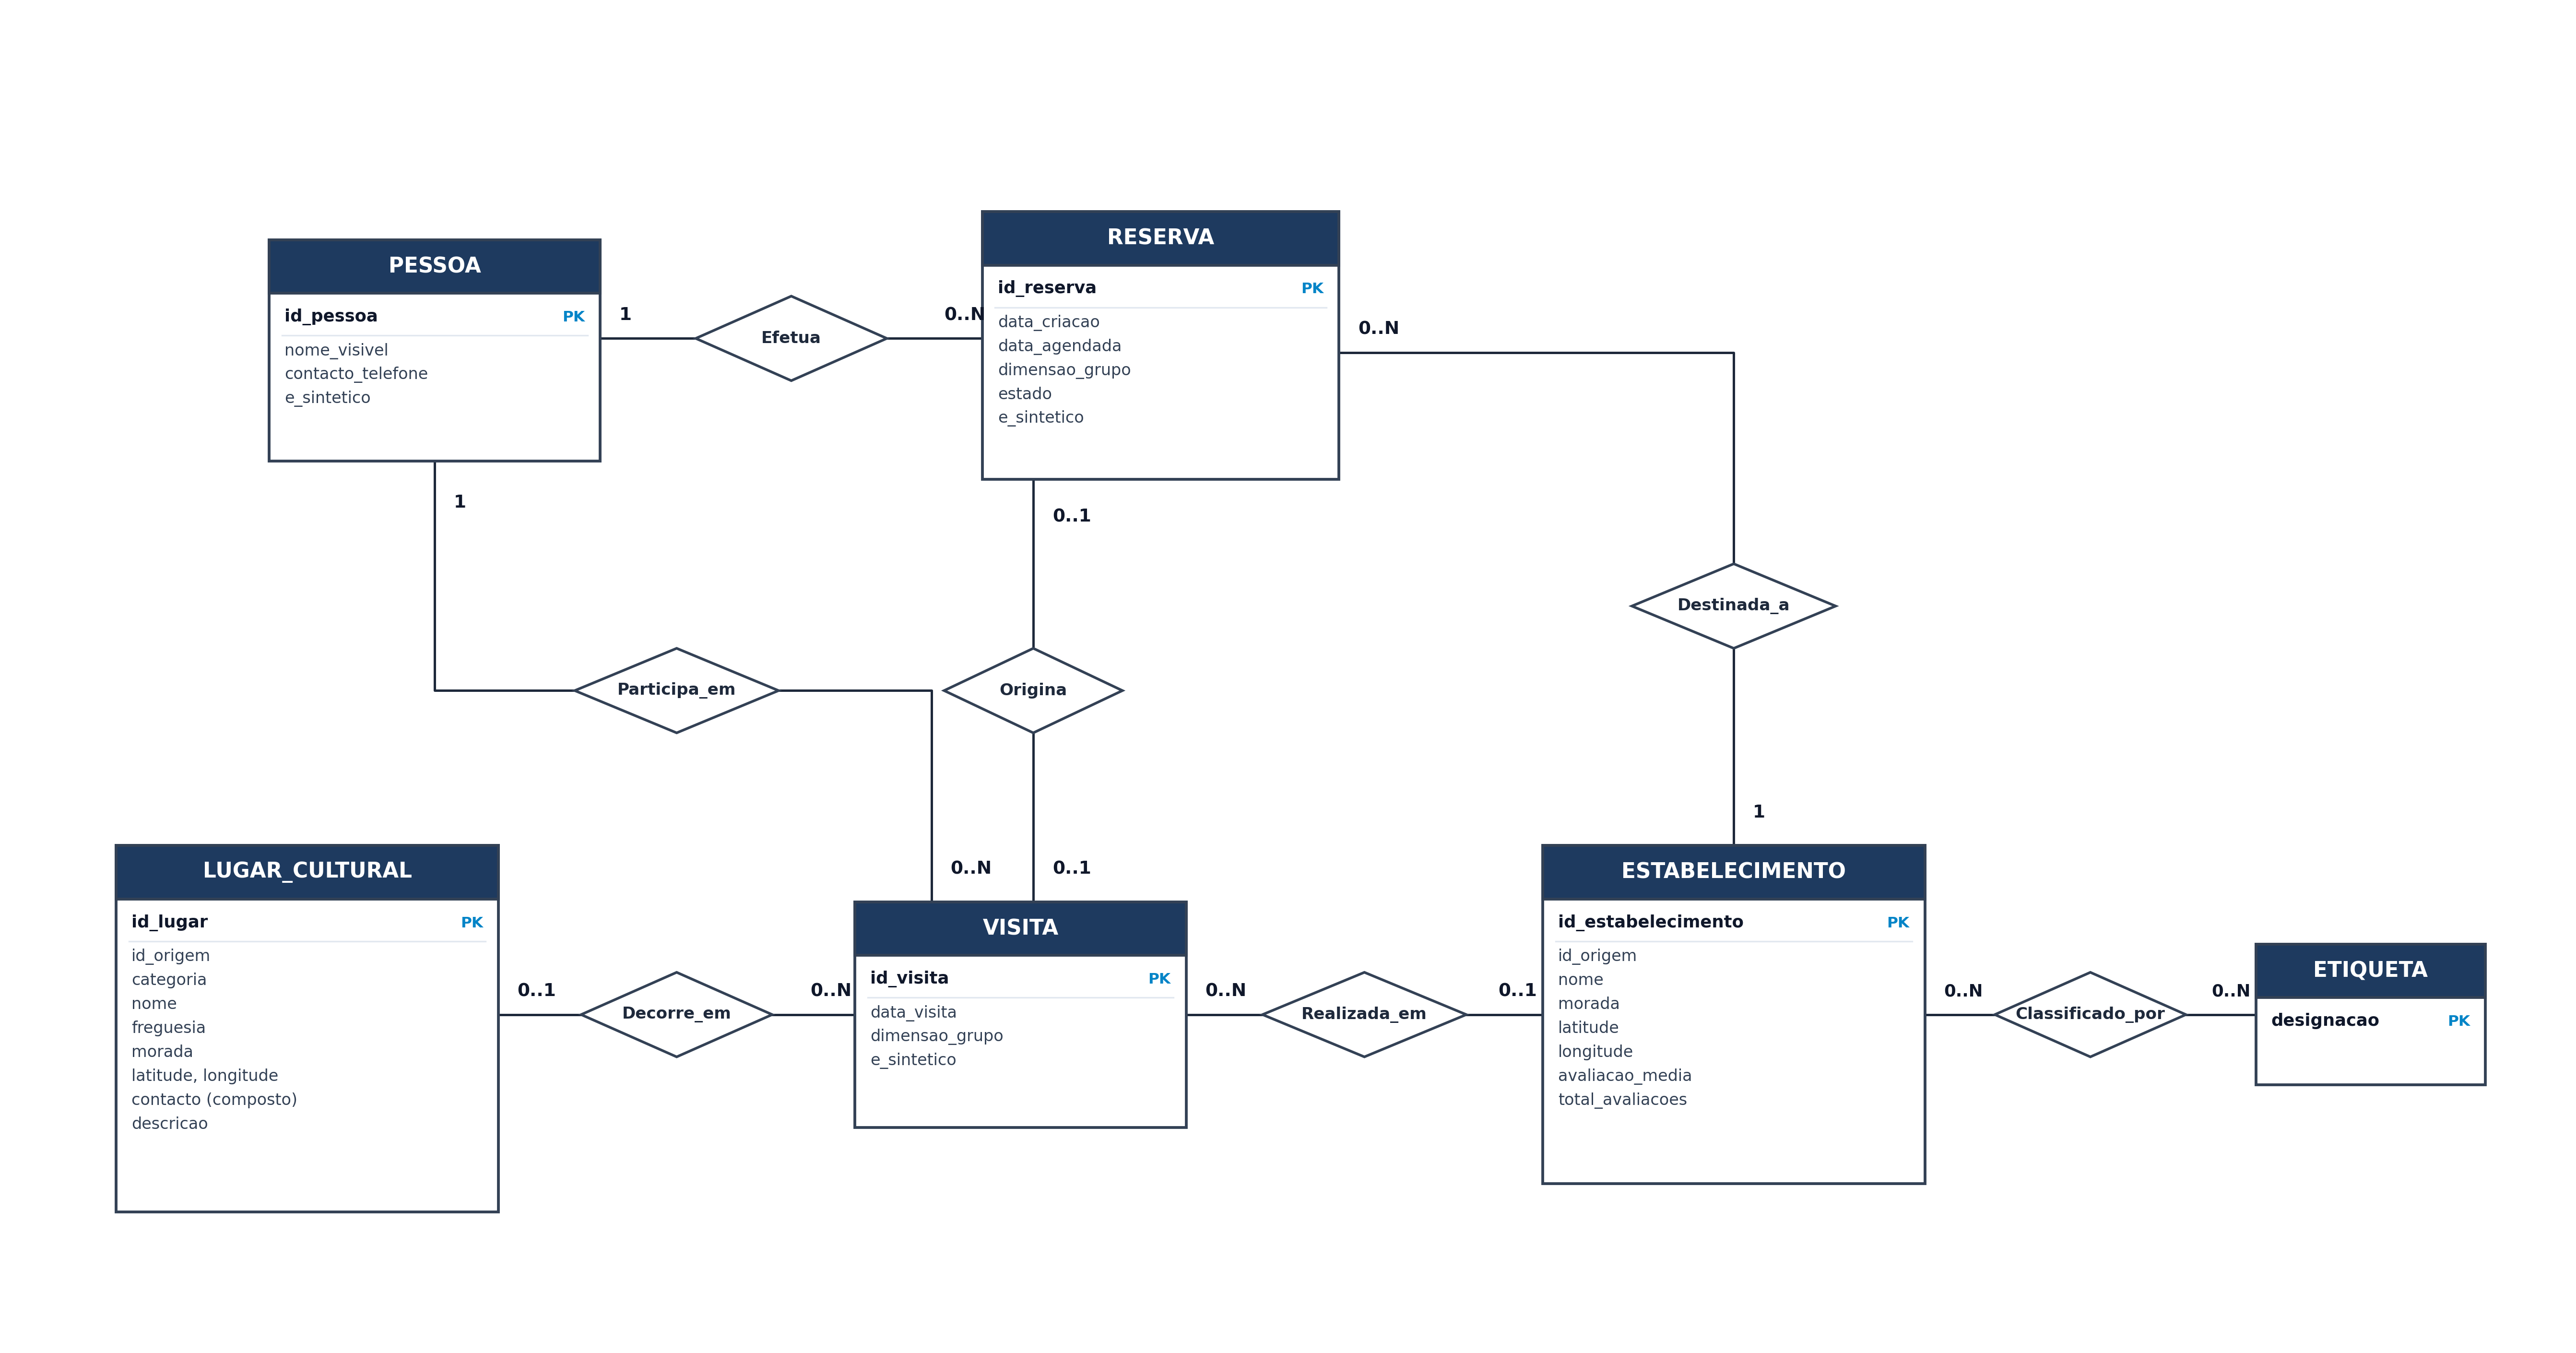
\includegraphics[width=\linewidth,height=0.84\textheight,keepaspectratio]{der_tiago.png}
\caption{Original ER diagram of the local Restaurant, Culture and Activity entities (Tiago Vailant). The English label key follows.}\label{fig:der}
\end{figure}\end{landscape}
\paragraph{English Label Key for Figure~\ref{fig:der}.}
The original diagram retains its Portuguese labels. \texttt{PESSOA} means Person; \texttt{RESERVA}, Reservation; \texttt{VISITA}, Visit; \texttt{ESTABELECIMENTO}, Establishment; \texttt{ETIQUETA}, Label; and \texttt{LUGAR\_CULTURAL}, Cultural Place. Relationship labels translate as follows: \emph{Efetua}, makes; \emph{Destinada\_a}, destined for; \emph{Origina}, gives rise to; \emph{Participa\_em}, participates in; \emph{Decorre\_em}, takes place at; \emph{Realizada\_em}, made at; and \emph{Classificado\_por}, classified by.

Attribute names use \texttt{id} for identifier and \texttt{id\_origem} for source identifier. The remaining labels mean: \texttt{nome\_visivel}, display name; \texttt{contacto\_telefone}, telephone contact; \texttt{e\_sintetico}, synthetic flag; \texttt{data\_criacao}, creation date; \texttt{data\_agendada}, scheduled date; \texttt{dimensao\_grupo}, group size; \texttt{estado}, status; \texttt{data\_visita}, visit date; \texttt{categoria}, category; \texttt{nome}, name; \texttt{freguesia}, parish; \texttt{morada}, address; \texttt{contacto}, contact (\texttt{composto} means composite); \texttt{descricao}, description; \texttt{avaliacao\_media}, average rating; \texttt{total\_avaliacoes}, review count; and \texttt{designacao}, label text. Latitude and longitude retain the same meaning in both languages. The logical schema below gives the corresponding implementation fields.

\paragraph{2. Relational Logical Model and Functional Dependencies (B1):}
The PostgreSQL relational schema \texttt{tiago\_\allowbreak{}lab} comprises five relations, with primary keys underlined and references indicated:
\begin{itemize}\raggedright
\item \texttt{ESTABLISHMENT}(\underline{establishment\_id}, source\_id, name, address, latitude, longitude, average\_rating, review\_count) --- \emph{UK:} \texttt{source\_\allowbreak{}id}
\item \texttt{ESTABLISHMENT\_\allowbreak{}LABEL}(\underline{establishment\_id}, \underline{label}) --- \emph{FK:} \texttt{establishment\_\allowbreak{}id} $\rightarrow$ \texttt{ESTABLISHMENT}
\item \texttt{PERSON}(\underline{person\_id}, display\_name, contact\_phone, is\_synthetic) --- \emph{UK:} \texttt{(\allowbreak{}display\_\allowbreak{}name,\allowbreak{} contact\_\allowbreak{}phone)}
\item \texttt{RESERVATION}(\underline{reservation\_id}, person\_id, establishment\_id, created\_at, scheduled\_at, party\_size, status, is\_synthetic) --- \emph{FKs:} \texttt{person\_\allowbreak{}id} $\rightarrow$ \texttt{PERSON}; \texttt{establishment\_\allowbreak{}id} $\rightarrow$ \texttt{ESTABLISHMENT}; \emph{UKs:} \texttt{(\allowbreak{}person\_\allowbreak{}id,\allowbreak{} establishment\_\allowbreak{}id,\allowbreak{} scheduled\_\allowbreak{}at)}; \texttt{(\allowbreak{}reservation\_\allowbreak{}id,\allowbreak{} person\_\allowbreak{}id,\allowbreak{} establishment\_\allowbreak{}id)}
\item \texttt{VISIT}(\underline{visit\_id}, person\_id, establishment\_id, cultural\_place\_id, reservation\_id, visited\_at, party\_size, is\_synthetic) --- \emph{FKs:} \texttt{person\_\allowbreak{}id} $\rightarrow$ \texttt{PERSON}; \texttt{establishment\_\allowbreak{}id} $\rightarrow$ \texttt{ESTABLISHMENT}; \texttt{(\allowbreak{}reservation\_\allowbreak{}id,\allowbreak{} person\_\allowbreak{}id,\allowbreak{} establishment\_\allowbreak{}id)} $\rightarrow$ \texttt{RESERVATION}; \emph{UKs:} \texttt{reservation\_\allowbreak{}id}; \texttt{(\allowbreak{}person\_\allowbreak{}id,\allowbreak{} visited\_\allowbreak{}at)}
\end{itemize}
\paragraph{3. Identifier and Key Semantics:}
\begin{itemize}\raggedright
\item \textbf{Establishment and Labels:} The natural Tripadvisor key (\texttt{source\_\allowbreak{}id UNIQUE}) is retained for traceability, while joins use the integer \texttt{establishment\_\allowbreak{}id}. The multivalued \texttt{cuisines} column is decomposed into associations keyed by \texttt{(\allowbreak{}establishment\_\allowbreak{}id,\allowbreak{} label)}. In this relation, the attributes form the key; in the remaining relations, descriptive attributes depend on the establishment, group representative or event key. Catalogue normalisation separates label associations from establishment attributes; the visit relation retains the controlled redundancy described below.
\item \textbf{Person (\texttt{PERSON}):} Restaurant bookings and cultural visits do not collect civil identity documents, and neither \texttt{display\_\allowbreak{}name} (namesakes \texttt{"Ana Exemplo"} in IDs \texttt{1} and \texttt{3}) nor \texttt{contact\_\allowbreak{}phone} (shared family number \texttt{"+351910000002"} in IDs \texttt{2} and \texttt{4}) is unique alone. Each group representative is therefore naturally identified by the composite candidate key \texttt{UNIQUE (\allowbreak{}display\_\allowbreak{}name,\allowbreak{} contact\_\allowbreak{}phone)}, while \texttt{person\_\allowbreak{}id} serves as the integer primary key for joins.
\item \textbf{Reservation and Visit:} The keys \texttt{reservation\_\allowbreak{}id} and \texttt{visit\_\allowbreak{}id} identify distinct reservation and visit occurrences, paired with natural composite candidate keys: \texttt{UNIQUE (\allowbreak{}person\_\allowbreak{}id,\allowbreak{} establishment\_\allowbreak{}id,\allowbreak{} scheduled\_\allowbreak{}at)} in \texttt{RESERVATION} (one booking per representative, establishment and scheduled instant) and \texttt{UNIQUE (\allowbreak{}person\_\allowbreak{}id,\allowbreak{} visited\_\allowbreak{}at)} in \texttt{VISIT} (no simultaneous visits by the same representative).
\end{itemize}
Each event key allows repeated reservations or visits by the same group representative to the same place at distinct timestamps. The \texttt{UNIQUE} constraint on the reservation identifier, group representative and establishment provides a superkey supporting the composite foreign key. For visits linked to a reservation, the group representative and establishment repeat the reservation values to allow declarative consistency checks; for walk-in visits, these values identify the event directly. This controlled redundancy and optional reference mean that primary keys alone do not establish 3NF.
\paragraph{4. PostgreSQL Physical Model:}
\begin{itemize}\raggedright
\item \textbf{Domains and Coordinates:} WGS84 bounds, \texttt{average\_\allowbreak{}rating} in $[0, 5]$ (\texttt{numeric(\allowbreak{}2,\allowbreak{}1)}) and mandatory coordinate pairing: \texttt{CHECK (\allowbreak{}(\allowbreak{}latitude IS NULL) = (\allowbreak{}longitude IS NULL))}.
\item \textbf{States and Chronology:} Status is restricted to \texttt{\{'confirmed',\allowbreak{} 'fulfilled',\allowbreak{} 'cancelled',\allowbreak{} 'no\_\allowbreak{}show'\}}, with the invariant \texttt{CHECK (\allowbreak{}created\_\allowbreak{}at <= scheduled\_\allowbreak{}at)}.
\item \textbf{Exclusive Arc and Composite FK:} In \texttt{VISIT}, \texttt{CHECK (\allowbreak{}num\_\allowbreak{}nonnulls(\allowbreak{}establishment\_\allowbreak{}id,\allowbreak{} cultural\_\allowbreak{}place\_\allowbreak{}id) = 1)} ensures a single destination; the composite FK to \texttt{RESERVATION}, together with \texttt{reservation\_\allowbreak{}id UNIQUE}, prevents a completed visit from diverging from its reservation's group representative or restaurant.
\end{itemize}
\paragraph{5. XML Logical and Physical Model in BaseX:}
\begin{itemize}\raggedright
\item \textbf{Hierarchy and Native Key:} The \texttt{<culturalCatalogue>} root groups 130 \texttt{<place>} elements with mandatory attributes \texttt{@id} (pattern \texttt{(\allowbreak{}museum|monument):.+}, uniqueness through \texttt{xs:key} \texttt{placeKey}), \texttt{@category} and \texttt{@sourceRef}, followed by \texttt{<name>}, \texttt{<location>} (\texttt{address}, \texttt{latitude}, \texttt{longitude}, \texttt{parish}), \texttt{<contact>} and \texttt{<description>}.
\item \textbf{Nullability and Cross-DBMS Link:} Contact and description subelements declare \texttt{nillable="true"} (\texttt{xsi:nil="true"}), distinguishing explicit absence from omission of \texttt{<fax>}. Column \texttt{visit.cultural\_\allowbreak{}place\_\allowbreak{}id} (B1) references \texttt{place/@id} (B2) across autonomous engines.
\end{itemize}
The XML schema also includes \texttt{sources/source} metadata, keyed by \texttt{sourceKey}, and the \texttt{placeSource} reference from \texttt{place/@sourceRef} to that key. The \texttt{sourceFields} block preserves raw source attributes. Quality checks also verify agreement between category, identifier prefix and source reference.

Reservation--visit rules are verified by audit queries: \texttt{fulfilled} status, a visit after reservation creation, matching group size and a visit for each fulfilled reservation. Cultural reference checks compare B1 against XML identifiers. Distinguishing declarative constraints from audits locates responsibility for each check.
The XSD is applied by the catalogue preparation and verification process. The BaseX database permits subsequent changes, which require those checks to be rerun; the schema is not automatically reapplied to every write. Raw \texttt{sourceFields} values are retained without specific validation. Agreement between category, source and identifier prefix is audited using XQuery. For contacts, checks measure structure and completeness; telephone normalisation in integrated queries follows the contract planned for P2.
\subsection{Gonçalo Serafim's Source Models (A1 and A2)}\label{subsec:modelos_goncalo}
\subsubsection{Conceptual Model and Identity}
The model in Figure~\ref{fig:der_goncalo} comprises Person, Owner, Accommodation, Review and Price Quote. Each owner corresponds to one person; a person may assume the owner role. An owner has one or more accommodations, and each accommodation has one owner. Each review has one author and one accommodation. An accommodation receives zero or more reviews and has zero or more quote families.

Person identifies the source account profile. The same account retains its key in the author and host roles. The link to Owner brings together document identification and activity indicators. Relationships use keys: \texttt{person\_\allowbreak{}id} derives from the original account; \texttt{owner\_\allowbreak{}id} identifies its owner role; \texttt{listing\_\allowbreak{}id} identifies the listing. The review key combines the listing and original comment identifier, in the form \texttt{R<listing>-<comment>}. Histories belong to the observed entity as multivalued composite attributes.

The document forms an alternate Owner key: issuing country, type and number, represented by \texttt{document\_\allowbreak{}key}. The technical key preserves references when document details are updated. The exercise maintains consistent document identification for each owner in each preparation run.

In the figure, indentation shows the components of a composite attribute; 1..N indicates a multivalued collection. In Price Quote, the monetary context, timestamp, received values and quality indicators belong to each observation. In Owner, the alternate key uses document country, type and number; nationality is a component of the document profile. Derived states use the reference dates specified in the logical model.
\begin{landscape}\begin{figure}[p]\centering
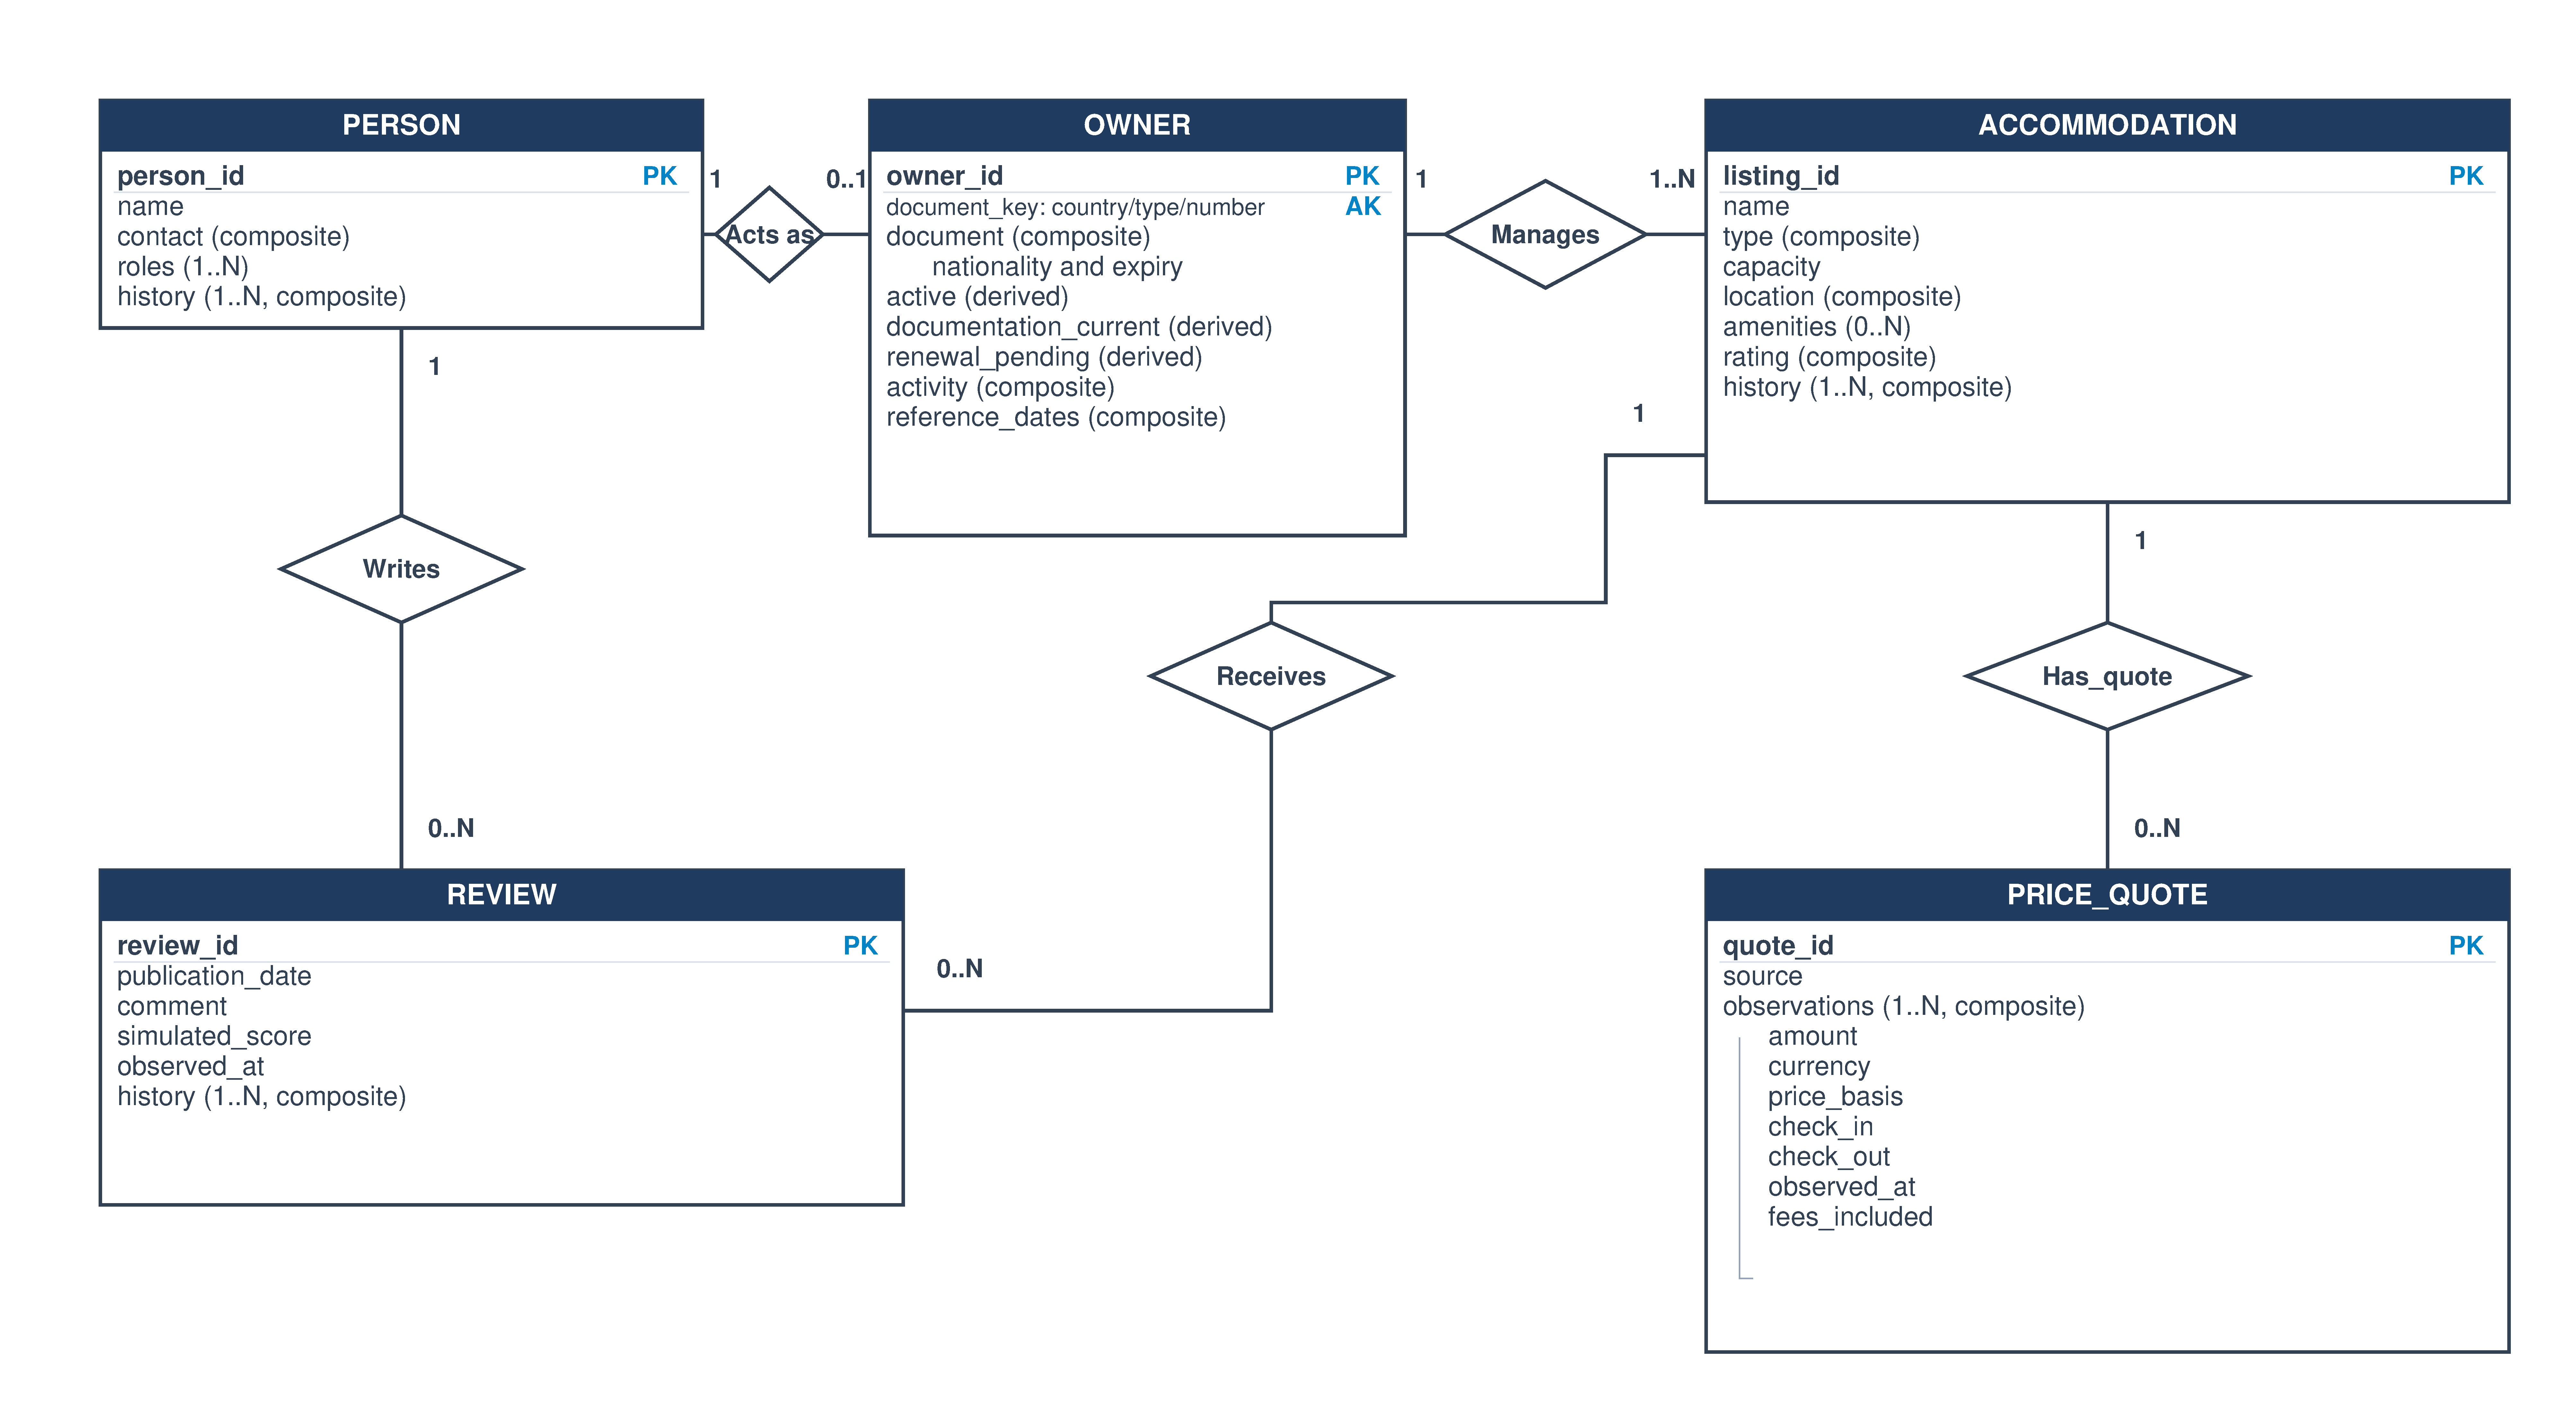
\includegraphics[width=\linewidth,height=0.84\textheight,keepaspectratio]{der_goncalo_owner_en.pdf}
\caption{ER diagram of the local Accommodation, Review, Owner and Price Quote entities (Gonçalo Serafim).}\label{fig:der_goncalo}
\end{figure}\end{landscape}
\subsubsection{Owner, Document and Derived States}
Owner references Person and brings together \texttt{identity\_\allowbreak{}document}, activity and the indicators \texttt{active}, \texttt{documentation\_\allowbreak{}up\_\allowbreak{}to\_\allowbreak{}date} and \texttt{needs\_\allowbreak{}renewal}. The activity block stores the number of accommodations, recent review count, latest known publication date, period start and assessment date.

Activity is calculated from logical reviews since 1 January 2025, summed across the owner's accommodations. A positive count determines \texttt{active = true}. Document validity compares the reference date with \texttt{expires\_\allowbreak{}on}: the document remains valid throughout its expiry date and requires renewal from the following day. Thus, an active owner may have an outstanding document renewal, and an inactive owner may hold up-to-date documentation.

The scenario generates Portuguese and British nationalities independently of the telephone contact's country. Synthetic Portuguese Citizen Card identifiers follow the official structure and check-digit rules\cite{cc_formato}, while British passport identifiers contain nine digits\cite{passport_formato}. Identifiers are stored as text, remain unique across owners and are explicitly distinguished from real personal data.

Document dates use the calendar domain 1900--2199, suitable for representing future expiry dates in the scenario. Document identifiers are critical information: preparation produces valid, unique numbers, and pre-validation rejects missing or invalid documents, documents shared by different accounts, and inconsistent documents for the same owner.

Persisted document indicators form a snapshot dated by \texttt{status\_\allowbreak{}as\_\allowbreak{}of}. Queries recalculate validity for the requested date, defaulting to the current date. Activity retains the assessment date of the prepared dataset. The two dates allow the currency of the indicators to be interpreted separately.
\subsubsection{A1 Logical and Physical Model}
The review index contains one record per logical review, bringing together its accommodation, author, publication date, comment, simulated score, history and quality indicators. A separate person index stores account profiles and contact information. Owner identification is maintained in A2 and represented consistently in A1.

Lexical search uses BM25 to rank matching comments and highlight relevant excerpts. Optional semantic search uses Qwen3-Embedding-4B to represent comments as 1\,024-dimensional vectors, compared using cosine similarity. Raw histories remain available for inspection, while searches operate on canonical values.
\subsubsection{A2 Logical and Physical Model}
The accommodation database organises information into four collections: accommodations, people, owners and price quotes.
\begin{description}
\item[\texttt{accommodation}.] Key \texttt{listing\_\allowbreak{}id}; references \texttt{owner\_\allowbreak{}id} and \texttt{host\_\allowbreak{}person\_\allowbreak{}id}; name, type, capacity, amenities, location, ratings, review summary and history. GeoJSON positions use longitude--latitude order.
\item[\texttt{people}.] Host account profiles, identified by \texttt{person\_\allowbreak{}id}, with name, contact country and national number, roles and observations. A1's contact representation includes the country calling code; A2 stores country and national number separately.
\item[\texttt{owners}.] Technical keys \texttt{owner\_\allowbreak{}id} and \texttt{person\_\allowbreak{}id}, document identification, activity, validity and assessment dates. Uniqueness is enforced on each of these references and on the document key.
\item[\texttt{price\_\allowbreak{}quotes}.] Key \texttt{quote\_\allowbreak{}id}, reference \texttt{listing\_\allowbreak{}id}, source and observation list. Each observation preserves its original, normalised values and quality indicators. Normalised amounts use Decimal128.
\end{description}
Strict validators check types and permitted fields. Canonical coordinates are both known or both null; valid locations have a \texttt{2dsphere} index. Canonical dates are BSON dates. Unique indexes protect keys, while load validation checks cross-document references and consistency of the owner projection in A1. Owner validation expressions check CC check digits, consistency between country, type and number, and agreement of derived states with stored counts and dates.
\subsubsection{Quotes and Query-Time Resolution}
The monetary context is the tuple \( (\text{amount},\text{currency},\text{check-in},\text{check-out},\text{basis},\text{fees}) \). A usable monetary observation has a finite, non-negative amount, currency in EUR/GBP/USD, and basis \texttt{unspecified}, \texttt{per\_\allowbreak{}night} or \texttt{per\_\allowbreak{}stay}. Dates and fee inclusion may remain unknown. Selection preserves the entire tuple of the chosen observation.

Under \texttt{agreement-only}, a quote is resolved when all usable tuples agree. Policy \texttt{latest-valid} accepts the same agreement case; where values differ, it requires known timestamps for every usable observation and agreement among observations at the latest timestamp. A conflicting tie or a conflict with incomplete chronology yields an \emph{unresolved} state. Absence of usable observations yields an \emph{unavailable} state.

The prepared source data retain reference amounts with basis \texttt{unspecified} and unknown fee inclusion. Queries with price limits compare this resolved amount in EUR. The catalogue's mean price represents the mean of these reference amounts. The additional \texttt{simulated} scenario declares nightly amounts and stay dates. Date-based searches compare requested dates with the context selected by the policy. Observations, including exact copies, remain available throughout the process.
